%\vspace{-5pt}
\section{Window Selection}
\label{sec:window}

\begin{figure}
  \centering
  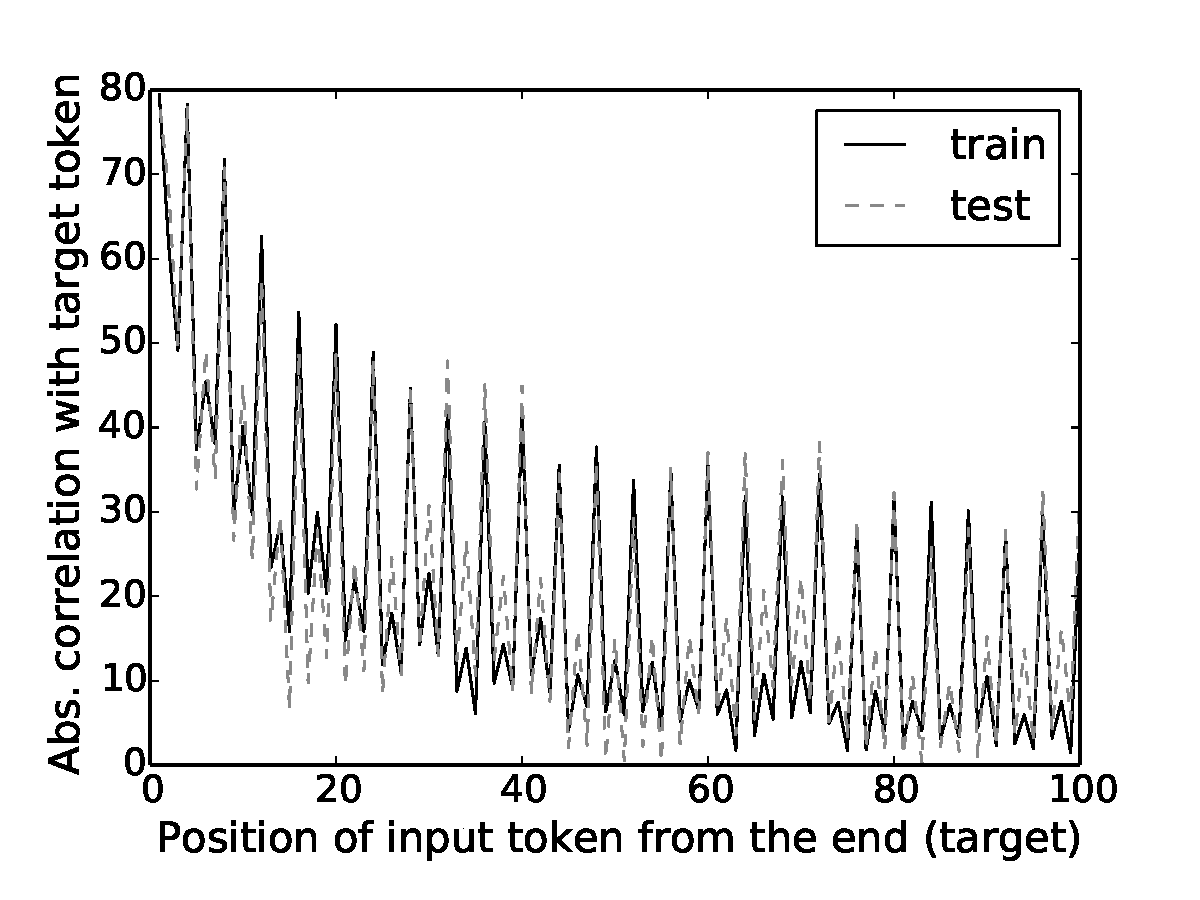
\includegraphics[width=\linewidth]{figs/correlation.pdf}
  \caption{Absolute value of correlation between input tokens and target token,
    as a function of position of a token from the target, for Linux source.}
  \label{fig:correlation}
\end{figure}

\noindent
To study the influence of tokens in an incomplete piece of code on the next
(target) token, we computed the correlation between the input tokens and the
target token.
Figure~\ref{fig:correlation} shows the result (scaled absolute correlation) for
codes that we train on and codes that we test on, for Linux
source code.
We compute the correlation between every token and preceding tokens, whenever
there are at least 100 tokens before the target.
The value of a key token is between 1 and $K$, and the value of a positional
token between $K+1$ and $K+W$, with $W=100$ here.
As we expected, the absolute value of correlation between input tokens and
target token gradually decreases as the distance between them increases.
However, interestingly, when an input token is 3 tokens or more away from the
target token, tokens that are even number of tokens away (tokens 4, 6, 8, ...
from the end) have a larger magnitude of correlation with the target token.
We think this is because special characters (operators) and words such as variable and
function names typically alternate. If other projects and languages
also exhibit a similar trend, we would like to see if we can improve
predictions by considering larger windows of preceding tokens, but after
removing tokens that are odd number of tokens away from the target token.
